% Options for packages loaded elsewhere
\PassOptionsToPackage{unicode}{hyperref}
\PassOptionsToPackage{hyphens}{url}
\PassOptionsToPackage{dvipsnames,svgnames,x11names}{xcolor}
%
\documentclass[
  letterpaper,
  DIV=11,
  numbers=noendperiod]{scrartcl}

\usepackage{amsmath,amssymb}
\usepackage{iftex}
\ifPDFTeX
  \usepackage[T1]{fontenc}
  \usepackage[utf8]{inputenc}
  \usepackage{textcomp} % provide euro and other symbols
\else % if luatex or xetex
  \usepackage{unicode-math}
  \defaultfontfeatures{Scale=MatchLowercase}
  \defaultfontfeatures[\rmfamily]{Ligatures=TeX,Scale=1}
\fi
\usepackage{lmodern}
\ifPDFTeX\else  
    % xetex/luatex font selection
\fi
% Use upquote if available, for straight quotes in verbatim environments
\IfFileExists{upquote.sty}{\usepackage{upquote}}{}
\IfFileExists{microtype.sty}{% use microtype if available
  \usepackage[]{microtype}
  \UseMicrotypeSet[protrusion]{basicmath} % disable protrusion for tt fonts
}{}
\makeatletter
\@ifundefined{KOMAClassName}{% if non-KOMA class
  \IfFileExists{parskip.sty}{%
    \usepackage{parskip}
  }{% else
    \setlength{\parindent}{0pt}
    \setlength{\parskip}{6pt plus 2pt minus 1pt}}
}{% if KOMA class
  \KOMAoptions{parskip=half}}
\makeatother
\usepackage{xcolor}
\setlength{\emergencystretch}{3em} % prevent overfull lines
\setcounter{secnumdepth}{-\maxdimen} % remove section numbering
% Make \paragraph and \subparagraph free-standing
\makeatletter
\ifx\paragraph\undefined\else
  \let\oldparagraph\paragraph
  \renewcommand{\paragraph}{
    \@ifstar
      \xxxParagraphStar
      \xxxParagraphNoStar
  }
  \newcommand{\xxxParagraphStar}[1]{\oldparagraph*{#1}\mbox{}}
  \newcommand{\xxxParagraphNoStar}[1]{\oldparagraph{#1}\mbox{}}
\fi
\ifx\subparagraph\undefined\else
  \let\oldsubparagraph\subparagraph
  \renewcommand{\subparagraph}{
    \@ifstar
      \xxxSubParagraphStar
      \xxxSubParagraphNoStar
  }
  \newcommand{\xxxSubParagraphStar}[1]{\oldsubparagraph*{#1}\mbox{}}
  \newcommand{\xxxSubParagraphNoStar}[1]{\oldsubparagraph{#1}\mbox{}}
\fi
\makeatother


\providecommand{\tightlist}{%
  \setlength{\itemsep}{0pt}\setlength{\parskip}{0pt}}\usepackage{longtable,booktabs,array}
\usepackage{calc} % for calculating minipage widths
% Correct order of tables after \paragraph or \subparagraph
\usepackage{etoolbox}
\makeatletter
\patchcmd\longtable{\par}{\if@noskipsec\mbox{}\fi\par}{}{}
\makeatother
% Allow footnotes in longtable head/foot
\IfFileExists{footnotehyper.sty}{\usepackage{footnotehyper}}{\usepackage{footnote}}
\makesavenoteenv{longtable}
\usepackage{graphicx}
\makeatletter
\def\maxwidth{\ifdim\Gin@nat@width>\linewidth\linewidth\else\Gin@nat@width\fi}
\def\maxheight{\ifdim\Gin@nat@height>\textheight\textheight\else\Gin@nat@height\fi}
\makeatother
% Scale images if necessary, so that they will not overflow the page
% margins by default, and it is still possible to overwrite the defaults
% using explicit options in \includegraphics[width, height, ...]{}
\setkeys{Gin}{width=\maxwidth,height=\maxheight,keepaspectratio}
% Set default figure placement to htbp
\makeatletter
\def\fps@figure{htbp}
\makeatother

\usepackage{lscape}
\newcommand{\blandscape}{\begin{landscape}}
\newcommand{\elandscape}{\end{landscape}}
\usepackage{caption}
\captionsetup[figure]{labelformat=empty}
\captionsetup[table]{labelformat=empty}
\usepackage{float}
\floatplacement{figure}{H}
\KOMAoption{captions}{tableheading}
\makeatletter
\@ifpackageloaded{caption}{}{\usepackage{caption}}
\AtBeginDocument{%
\ifdefined\contentsname
  \renewcommand*\contentsname{Table of contents}
\else
  \newcommand\contentsname{Table of contents}
\fi
\ifdefined\listfigurename
  \renewcommand*\listfigurename{List of Figures}
\else
  \newcommand\listfigurename{List of Figures}
\fi
\ifdefined\listtablename
  \renewcommand*\listtablename{List of Tables}
\else
  \newcommand\listtablename{List of Tables}
\fi
\ifdefined\figurename
  \renewcommand*\figurename{Figure}
\else
  \newcommand\figurename{Figure}
\fi
\ifdefined\tablename
  \renewcommand*\tablename{Table}
\else
  \newcommand\tablename{Table}
\fi
}
\@ifpackageloaded{float}{}{\usepackage{float}}
\floatstyle{ruled}
\@ifundefined{c@chapter}{\newfloat{codelisting}{h}{lop}}{\newfloat{codelisting}{h}{lop}[chapter]}
\floatname{codelisting}{Listing}
\newcommand*\listoflistings{\listof{codelisting}{List of Listings}}
\makeatother
\makeatletter
\makeatother
\makeatletter
\@ifpackageloaded{caption}{}{\usepackage{caption}}
\@ifpackageloaded{subcaption}{}{\usepackage{subcaption}}
\makeatother

\ifLuaTeX
  \usepackage{selnolig}  % disable illegal ligatures
\fi
\usepackage{bookmark}

\IfFileExists{xurl.sty}{\usepackage{xurl}}{} % add URL line breaks if available
\urlstyle{same} % disable monospaced font for URLs
\hypersetup{
  colorlinks=true,
  linkcolor={RoyalBlue},
  filecolor={Maroon},
  citecolor={Blue},
  urlcolor={RoyalBlue},
  pdfcreator={LaTeX via pandoc}}


\author{}
\date{}

\begin{document}


\section{Project: PollObs (no title for
now)}\label{project-pollobs-no-title-for-now}

\emph{Provisional author position:}

Jose B. Lanuza\textsuperscript{1}, Henriette F.
Morgenroth\textsuperscript{1}, Raymond Umazekabiri\textsuperscript{1},
Marc Hoffmann\textsuperscript{1}, Panagiotis
Theodorou\textsuperscript{1,2}, Robert Paxton\textsuperscript{1,2},
Isabell Hensen\textsuperscript{1,2}, Robert
Rauschkolb\textsuperscript{1,3}, Christine
Römermann\textsuperscript{1,3}, Oliver Schweiger \textsuperscript{1,5},
Martin Freiberg\textsuperscript{1,4}, Alfonso
Allen-Perkins\textsuperscript{6}, Tiffany Knight\textsuperscript{1}

\emph{Affiliations}

\begin{enumerate}
\def\labelenumi{\arabic{enumi}.}
\tightlist
\item
  German Centre for Integrative Biodiversity Research (iDiv)
  Halle-JenaLeipzig, Puschstr. 4, 04103 Leipzig, Germany
\item
  Institute for Biology, Martin-Luther-UniversityHalle-Wittenberg, Hoher
  Weg 8, 06120 Halle (Saale), Germany
\item
  Institute of Ecology and Evolution with Herbarium Haussknecht and
  Botanical Garden, Friedrich Schiller University Jena, Jena, Germany
\item
  Systematic Botany and Functional Biodiversity/Botanical Garden,
  Institute of Biology, Leipzig University, Johannisallee 21-23, 04103,
  Leipzig, Germany
\item
  UFZ-Helmholtz Centre for Environmental Research, Department of
  Community Ecology, 06120 Halle, Germany
\item
  Departamento de Ingeniería Eléctrica, Electrónica, Automática y Física
  Aplicada, ETSIDI, Universidad Politécnica de Madrid, 28040 Madrid,
  Spain.
\end{enumerate}

\section{Abstract}\label{abstract}

Flowering plants exhibit an astonishing diversity of reproductive
structures, which shapes how they interact with their pollinators.
However, to what extent reproductive traits or other drivers like
phenology and species abundances shape plant-pollinator interactions is
still an open question. To disentangle the relative effects of species
phenology, abundances and traits in plant-pollinator interactions, we
compared pollinator visitation rates, diet breath, specialization from
plant species that vary in reproductive traits, phenology and
abundances. To do this, we observed plant-pollinator interactions for a
whole flowering season in three different botanical gardens located in
an urban setting. We anticipate that the ecological role of the
different plant and pollinator species are largely driven by their
phenological overlap and abundance, and only certain taxonomic groups
are strongly influenced by trait matching processes. Our results
highlight the relevance of considering multiple mechanisms to understand
plant-pollinator interactions.

\section{Main objective}\label{main-objective}

Explore how traits, phenology and abundances shape species interactions
in three botanical gardens from Germany.

Pending tasks:

\begin{itemize}
\item
  Clean trait and phenology data for plants
\item
  Get Pollinator phenology and traits
\item
  Easy things to check: alpha, beta and gamma diversity of pollinators
  across the three gardens.
\end{itemize}

\section{Methods}\label{methods}

WRITE XXXXX

\section{The data has an important temporal
component}\label{the-data-has-an-important-temporal-component}

In Figure 1 we can see in a color coded NMDS the strong temporal
component of the composition across gardens and different taxonomic
levels.

\begin{figure}[H]

{\centering 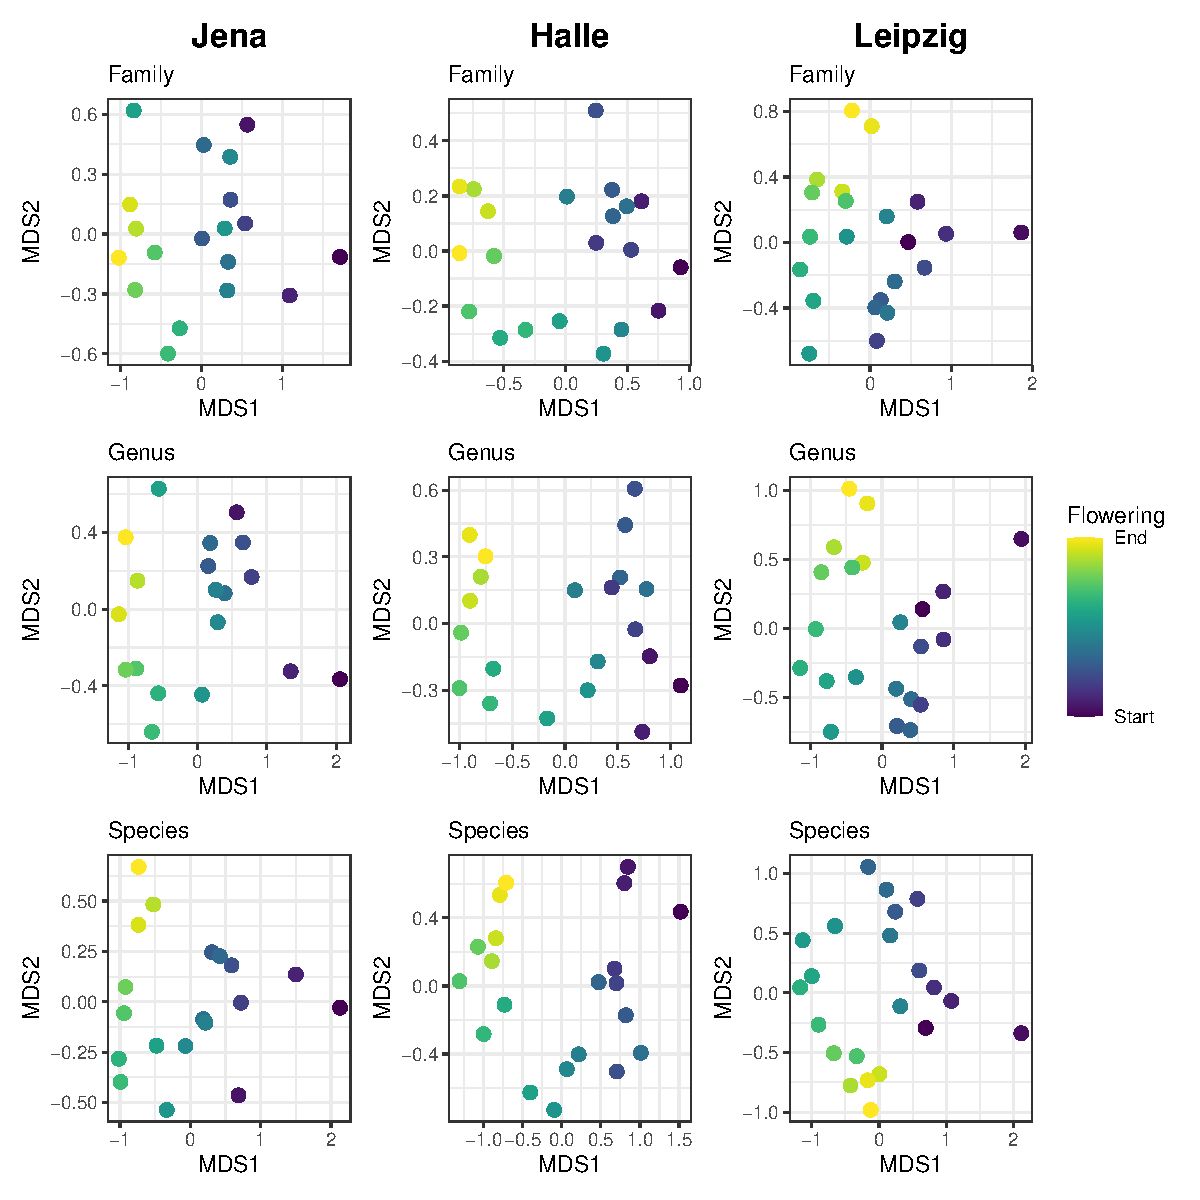
\includegraphics{Working_file_files/figure-pdf/unnamed-chunk-2-1.pdf}

}

\caption{\textbf{Figure 1}. Non-metric multidimensional scaling (NMDS)
of the pollinator community composition by sampling day in the three
gardens at family, genus and species level.}

\end{figure}%

\newpage

\section{Plant phenologies}\label{plant-phenologies}

The phenology of plants and pollinators was monitored weekly on each of
the three gardens. Unlike plants, pollinator phenology relies on
`stochastic' interaction obervations that may not represent their
complete flying period. Thus, we built a comprehensive flying period of
all pollinators by retrieving GBIF records for all observed floral
visitors during the sampling year. In addition, this download was
limited by area, where we considered a rectangular shape that extends
more on the longitude range than the latitude one, as we expect more
homogeneous environmental conditions in the former (\textbf{Figure X}).

\begin{figure}[H]

{\centering 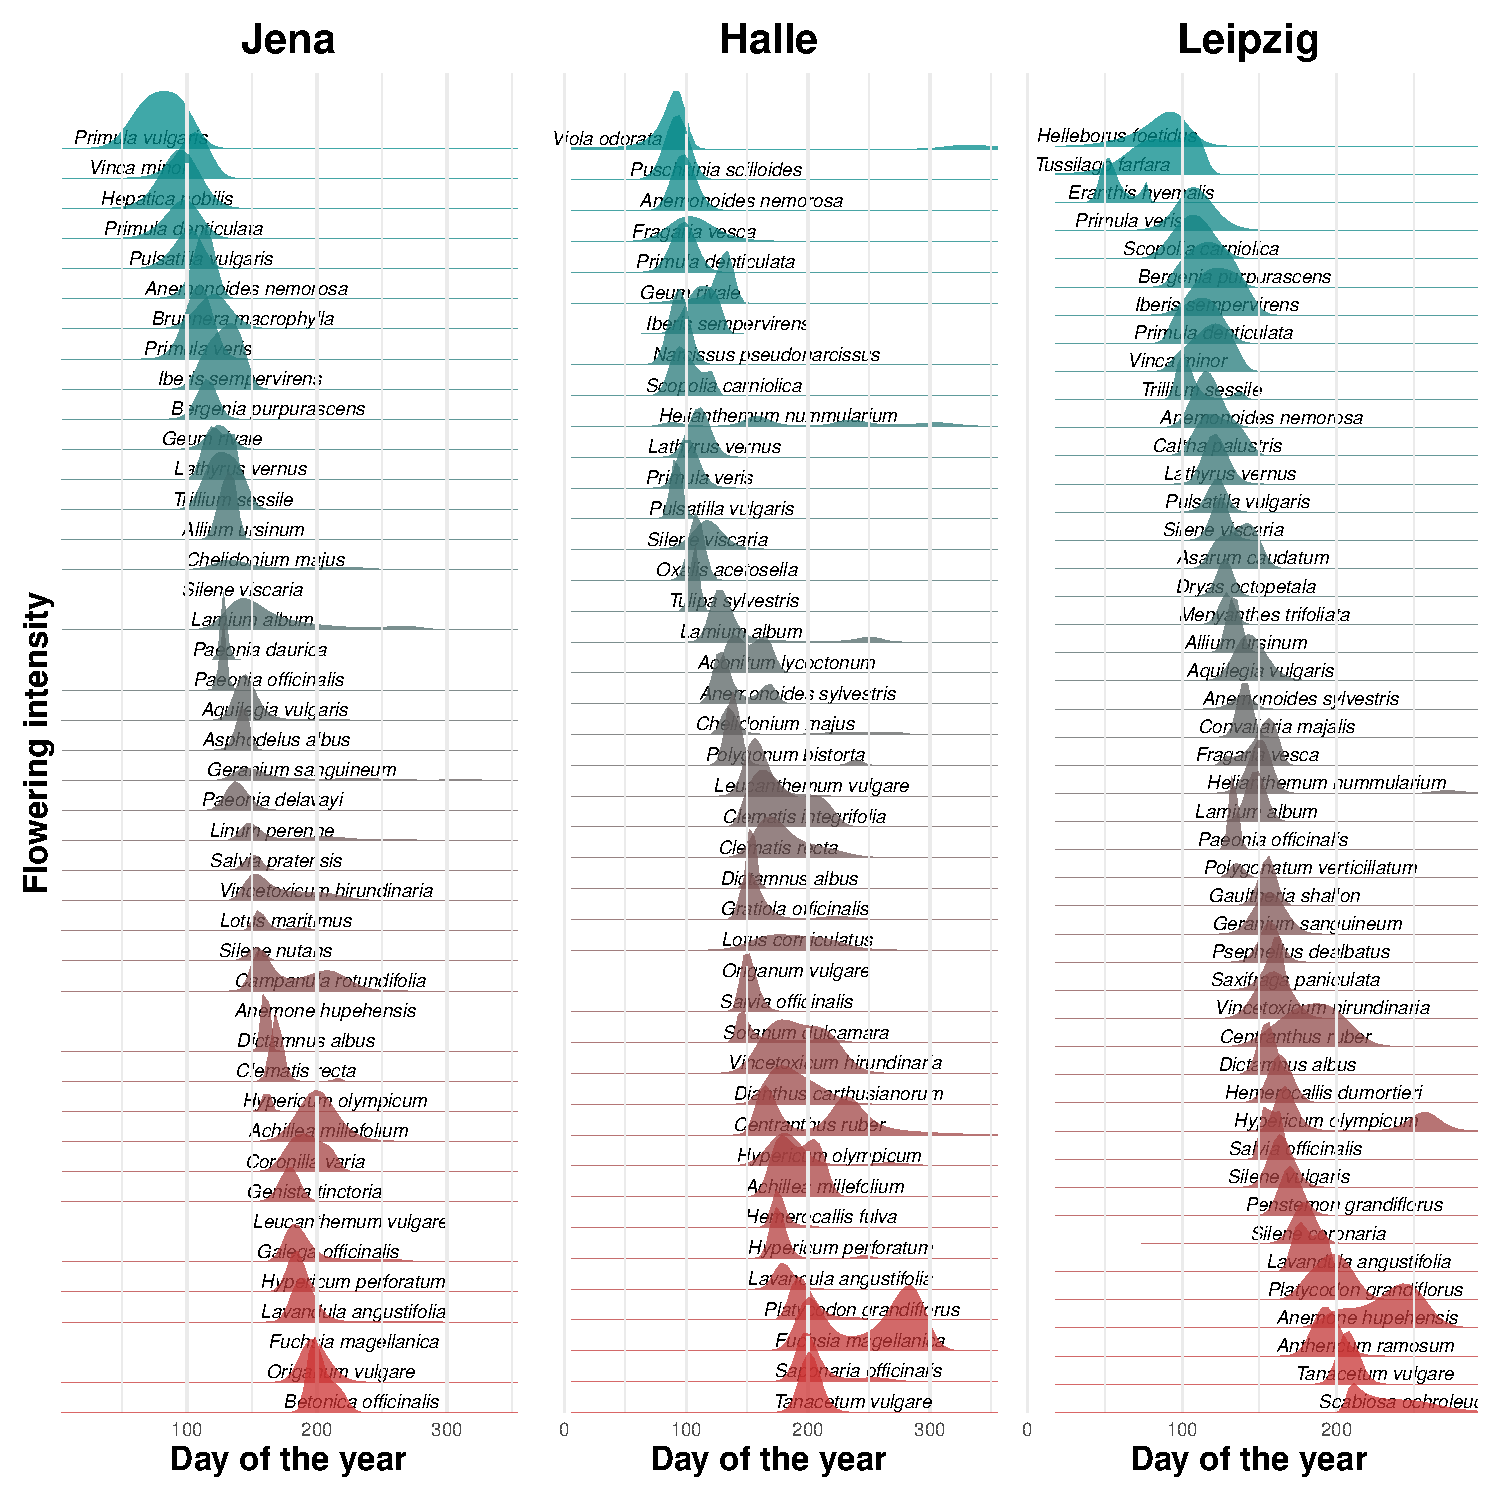
\includegraphics{Working_file_files/figure-pdf/unnamed-chunk-3-1.pdf}

}

\caption{\textbf{Figure 2}.}

\end{figure}%




\end{document}
